\documentclass[9pt]{beamer}
\usetheme{Boadilla}
\usepackage{tikz}
 \usepackage[english]{babel}
 \usepackage{amsmath}
 \usepackage{amsfonts}
 \usepackage{amssymb}
 \usepackage{amsthm}
 \usepackage{array}
 \newcommand{\tabitem}{%
  \usebeamertemplate{itemize item}\hspace*{\labelsep}}
 \usepackage{mathtools}
 \DeclarePairedDelimiterX{\inp}[2]{\langle}{\rangle}{#1, #2}
 \usepackage[utf8]{inputenc}
 \usepackage{dsfont}
 \usetikzlibrary{patterns}
 \usepackage{graphicx}
 \graphicspath{{"../Output/"}}
 \usepackage[export]{adjustbox}
 \usepackage{mathrsfs}
 \usepackage{bbold}
\usetikzlibrary{mindmap,trees,shadows}
\usepackage{caption}
\usepackage{tabularx}
\usepackage{booktabs}
\usepackage{caption}
\usepackage{changepage}
\usepackage{subcaption}
\usepackage{import}
\usepackage{hyperref}
% \usepackage{apacite}
\usepackage{listings}
\captionsetup[figure]{font=scriptsize}
\newcommand{\MYhref}[3][blue]{\href{#2}{\color{#1}{#3}}}%
\usepackage{hyperref} 
            \hypersetup{backref=true,       
                    pagebackref=true,               
                    hyperindex=true,                
                    colorlinks=true,                
                    breaklinks=true,                
                    urlcolor= blue,                
                    linkcolor= blue,                
                    bookmarks=true,                 
                    bookmarksopen=false,
                    citecolor=blue,
                    linkcolor=blue,
                    filecolor=blue,
                    citecolor=blue,
                    linkbordercolor=blue
}


\makeatletter
\def\input@path{{"../Output/"}}
\makeatother

% \usepackage{biblatex}
% \usepackage{natbib}
\usepackage[round]{natbib}
\bibliographystyle{unsrtnat}

\title{M2 Masters Thesis}
\subtitle{Options Portfolio Optimization under GARCH}
\author{Andrew Boomer}
\date{\today}

\begin{document}

\frame{\titlepage}

\begin{frame}{Introduction}
    \begin{itemize}
        \item This thesis investigates the topic of portfolio selection/optimization, which originates with the seminal paper of \cite{markowitz}.
        \item Standard portfolio selection optimizes a set of real weights on a basket of stocks
        \item I extend this topic through replacing a basket of stocks with a basket of options on the S\&P500, and the use of a GARCH volatility model.
    \end{itemize}
\end{frame}

\begin{frame}{Problem Statement}
    \begin{itemize}
        \item I use S\&P500 options data from the Chicago Board of Exchange (CBOE) spanning from January 2019 to May 2021.
        \item Following \cite{faias2017optimal}, I use a constant relative risk aversion (CRRA) utility function to optimize next period wealth.
        \item Next period wealth is reformulated in terms of the weighted sum of simulated option returns.
    \end{itemize}
\end{frame}

\begin{frame}{Motivation}
    \begin{itemize}
        \item In this research, I aim to set the theoretical modeling framework of an algorithm trading in the real markets. 
        \item With this foundation, I employ portfolio selection techniques found in the literature, while diving further into the practical discussion.
        \item This paper can also be used a baseline for a more in depth comparison of different volatility or returns prediction models.
    \end{itemize}
\end{frame}

\begin{frame}{Previous Literature}
    \begin{itemize}
        \item \cite{markowitz} employed a mean-variance model to select a portfolio of stocks.
        \item Multiple papers have addressed portfolio selection with options, including \cite{zhao2018markowitz} and \cite{faias2017optimal}.
        \item This thesis builds off the work of \cite{faias2017optimal}, who approach portfolio selection with options using a returns simulation framework based on ad-hoc volatility estimation.
    \end{itemize}
\end{frame}

\begin{frame}{Methodology}
I assume that the log returns follow a normal distribution with a time varying volatility term, which is modeled by a GARCH(1, 1) process. Formally:

\begin{align}
\nonumber y_{t} &= \sigma_{t} \epsilon_{t} \quad \epsilon_{t} \sim iid.N(0, 1)
\\ \nonumber \sigma_{t}^{2} &= \omega + \alpha y_{t - 1}^{2} + \beta \sigma_{t - 1}^{2}
\\ \nonumber & \omega > 0 \ \ \alpha, \beta \geq 0
\end{align}
\end{frame}

\begin{frame}{Methodology}
Formally, in this paper I optimize the wealth of the next period $A_{t + 1}$
\[\max_{\mathbf{W}_{t}} E[U(A_{t+1})|F_{t}]\]
Where $F_{t}$ as the available information at time $t$, $E$ is the expectation operator. $\mathbf{W}_{t}$ is the vector of allocated weights. The optimization is done via a simulation of the next period wealth $A_{t+1}^{n}$. This returns a vector of optimized weights $\mathbf{W}_{t}^{*}$.

\vspace{1cm}
Where $\gamma$ is the CRRA risk aversion parameter, the utility function U is:
\[U(A)=\left\{\begin{array}{ll}\frac{1}{1-\gamma} A^{1-\gamma}, & \text { if } \gamma \neq 1 \\ \log (A), & \text { if } \gamma=1\end{array}\right.\]
\end{frame}

\begin{frame}{Methodology}
    \begin{itemize}
        \item Option returns are calculated under a hold until expiration strategy, wherein after the initial trade, the trader cannot further adjust the portfolio.
        \item The model uses a CRRA expected utility function rather than the traditional mean-variance framework.
        \item $\gamma$ is set to 10, higher than 4 found in \cite{bliss2004option}, to induce shrinkage in $\mathbf{W}_{t}^{*}$.
    \end{itemize}
\end{frame}

\begin{frame}{Methodology}
Standardized returns based on the fitted conditional volatility series are $\hat{\epsilon}_{t} = \frac{y_{t}}{\hat{\sigma_{t}}}$. Simulated log returns are generated using a bootstrapped distribution of historic $\hat{\epsilon}_{t}$.

\[\tilde{y}^{n}_{t + h} = \hat{\sigma}_{t + h} \tilde{\epsilon}^{n}_{t + h} \quad \forall n \in N \ and \ \forall h \in T - t\]

\vspace{1cm}

Simulated option returns are calculated from simluated prices $S_{t + h|t+h-1}^{n} = S_{t + h - 1} e^{\tilde{y}_{t + h}^{n}}$.
\noindent
\begin{align} 
\nonumber C_{t+1 \mid t}^{n}(k) &= \max (S_{t+1 \mid t}^{n} - k, 0) \quad \quad k = K_{t, c_{1}}, \cdots, K_{t, c_{C}} 
\\ \nonumber P_{t+1 \mid t}^{n}(k) &= \max (k - S_{t+1 \mid t}^{n}, 0) \quad \quad k = K_{t, p_{1}}, \cdots, K_{t, p_{P}}
\\ \nonumber r_{t+1 \mid t, c}^{n}(k) &= \frac{C_{t+1 \mid t}^{n}(k)}{C_{t, k}} - 1 \quad \quad k = K_{t, c_{1}}, \cdots, K_{t, c_{C}}
\\ \nonumber r_{t+1 \mid t, p}^{n}(k) &= \frac{P_{t+1 \mid t}^{n}(k)}{P_{t, k}} - 1 \quad \quad k = K_{t, p_{1}}, \cdots, K_{t, p_{P}}
\end{align}
\end{frame}

\begin{frame}{Methodology}
Simulated next period wealth is formulated as current wealth times the simulated total return of the basket of options, dependent on the choice variable $\mathbf{W}_{t}$

\[A_{t+1 \mid t}^{n} = A_{t}(1 + rp_{t + 1 \mid t}^{n}(\mathbf{W}_{t}))\]

This quantity is used to optimize $\mathbf{W}_{t}$ based on the empirical mean of N simulations, which is independent of current wealth $A_{t}$.
\end{frame}

\begin{frame}{Results}
\begin{figure}[H]
\captionsetup{width=10cm, skip=0pt}
    \begin{center}
        \caption{\\ \textbf{Portfolio Optimization Returns} \rule{10cm}{0.5pt}\\ \footnotesize{\textit{Histogram of portfolio optimization returns is shown. The time period is January 2019 to May 2021.}}}
        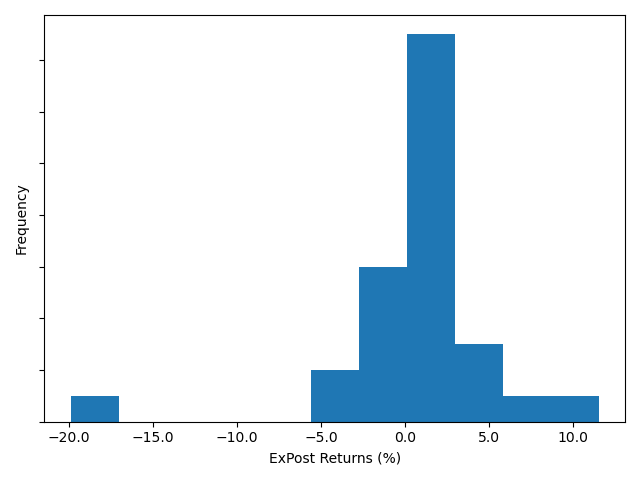
\includegraphics[width=7cm]{Graphs/Fig4_OOPSRet.png}
        \label{fig:Fig4_OOPSRet}
    \end{center}
\end{figure}
\end{frame}

\begin{frame}{Results}
\begin{figure}[H]
\begin{center}
\captionsetup{width=12cm, skip=5pt}
\caption{\\ \textbf{ExPost Results vs. S\&P500} \rule{12cm}{0.5pt}\\ \footnotesize{\textit{Summary of returns, portfolio optimization vs. S\&P500, along with graph of cumulative returns including risk-free asset. Mean, Std, Min, and Max are percentages. Period spans from January 2019 to May 2021.}}}
    \begin{minipage}{0.53\linewidth}
        \centerline{\begin{tabular}{lrrrrrrr}
\hline
         &   Mean &   Std &   Min &   Max &   Skew &   Kurtosis &   SR \\
\hline
 S\&P 500 &    1.8 &   4.7 & -19.1 &   6.3 &  -3.14 &      11.59 & 0.38 \\
 ExPost  &    0.7 &   5.0 & -19.9 &  11.5 &  -2.22 &       9.15 & 0.15 \\
\hline
\end{tabular}}
    \end{minipage}
    \begin{minipage}{0.8\linewidth}
        \begin{center}
            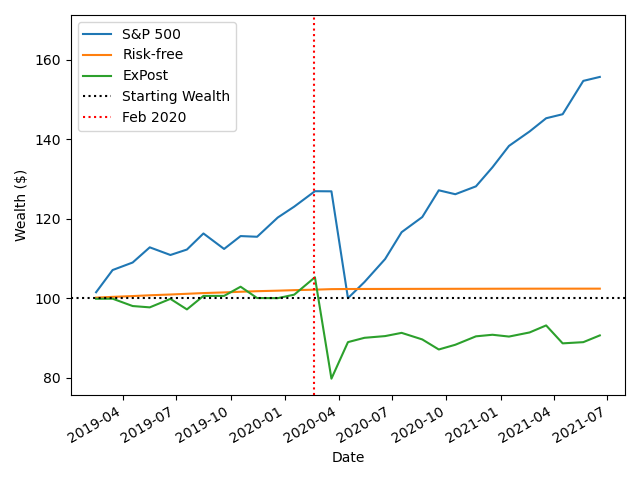
\includegraphics[width=7cm]{Graphs/Cum_Returns.png}
        \end{center}
    \end{minipage}
\label{fig:Results}
\end{center}
\end{figure}
\end{frame}

\begin{frame}{Results}
\begin{figure}[H]
\captionsetup{width=11cm, skip=0pt}
    \begin{center}
        \caption{\\ \textbf{Portfolio Optimization Weights by Contract} \rule{11cm}{0.5pt}\\ \footnotesize{\textit{Optimized weights from portfolio optimization are shown by option type, as well as for the call-put difference and risk-free assset. The time period is January 2019 to May 2021.}}}
        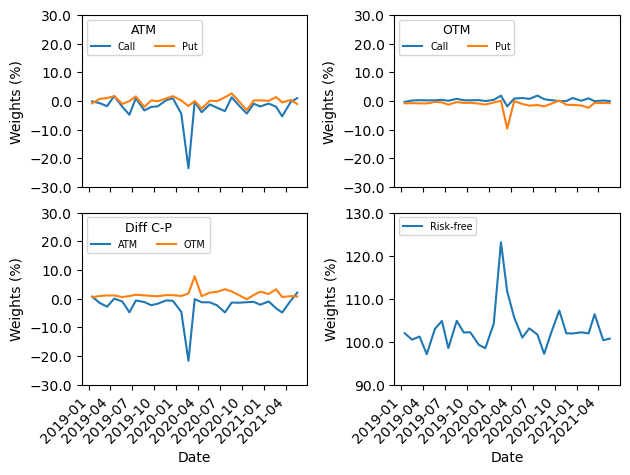
\includegraphics[width=7cm]{Graphs/WeightsPlot.png}
        \label{fig:Weights}
    \end{center}
\end{figure}
\end{frame}

\begin{frame}{Conclusion}
    \begin{itemize}
        \item Portfolio optimization returns show a sharpe ratio of -0.03 vs. 0.33 for the underlying S\&P500 in the time period.
        \item The ex-post returns do, however, show a lower skew and kurtosis, meaning the returns are closer to normality, even with the Covid months.
        \item Removing February and March of 2020 results in a sharpe ratio of 0.14. These months represent 6\% of the sample, so a larger sample with less weight on these months may impact results.
    \end{itemize}
\end{frame}

\begin{frame}
\begin{center}
\large{Thank you for listening!}
\end{center}
\end{frame}

\begin{frame}{References}
% \nocite{*}
\bibliography{References}    
\end{frame}

\end{document}